%%%%%%%%%%%%%%%%%%%%%%%%%%%%%%%%%%%%%%%%%
% Journal Article
% LaTeX Template
% Version 1.3 (9/9/13)
%
% This template has been downloaded from:
% http://www.LaTeXTemplates.com
%
% Original author:
% Frits Wenneker (http://www.howtotex.com)
%
% License:
% CC BY-NC-SA 3.0 (http://creativecommons.org/licenses/by-nc-sa/3.0/)
%
%%%%%%%%%%%%%%%%%%%%%%%%%%%%%%%%%%%%%%%%%

%----------------------------------------------------------------------------------------
%	PACKAGES AND OTHER DOCUMENT CONFIGURATIONS
%----------------------------------------------------------------------------------------

\documentclass[twoside]{article}

\usepackage{lipsum} % Package to generate dummy text throughout this template

\usepackage{fixltx2e}
\usepackage{graphicx}
\usepackage[sc]{mathpazo} % Use the Palatino font
\usepackage[T1]{fontenc} % Use 8-bit encoding that has 256 glyphs
\linespread{1.05} % Line spacing - Palatino needs more space between lines
\usepackage{microtype} % Slightly tweak font spacing for aesthetics

\usepackage[hmarginratio=1:1,top=32mm,columnsep=20pt]{geometry} % Document margins
\usepackage{multicol} % Used for the two-column layout of the document
\usepackage[hang, small,labelfont=bf,up,textfont=it,up]{caption} % Custom captions under/above floats in tables or figures
\usepackage{booktabs} % Horizontal rules in tables
\usepackage{float} % Required for tables and figures in the multi-column environment - they need to be placed in specific locations with the [H] (e.g. \begin{table}[H])
\usepackage{hyperref} % For hyperlinks in the PDF

\usepackage{lettrine} % The lettrine is the first enlarged letter at the beginning of the text
\usepackage{paralist} % Used for the compactitem environment which makes bullet points with less space between them

\usepackage{abstract} % Allows abstract customization
\renewcommand{\abstractnamefont}{\normalfont\bfseries} % Set the "Abstract" text to bold
\renewcommand{\abstracttextfont}{\normalfont\small\itshape} % Set the abstract itself to small italic text

\usepackage{titlesec} % Allows customization of titles
\renewcommand\thesection{\Roman{section}} % Roman numerals for the sections
\renewcommand\thesubsection{\Roman{subsection}} % Roman numerals for subsections
\titleformat{\section}[block]{\large\scshape\centering}{\thesection.}{1em}{} % Change the look of the section titles
\titleformat{\subsection}[block]{\large}{\thesubsection.}{1em}{} % Change the look of the section titles

\usepackage{fancyhdr} % Headers and footers
\pagestyle{fancy} % All pages have headers and footers
\fancyhead{} % Blank out the default header
\fancyfoot{} % Blank out the default footer
\fancyhead[C]{Bubble Break $\bullet$ October 2013 $\bullet$} % Custom header text
\fancyfoot[RO,LE]{\thepage} % Custom footer text

%----------------------------------------------------------------------------------------
%	TITLE SECTION
%----------------------------------------------------------------------------------------

\title{\vspace{-15mm}\fontsize{24pt}{10pt}\selectfont\textbf{Comparison of Different Strategies to solve Bubble Break}} % Article title

\author{
\large
\textsc{Harsimran Singh}\\%\thanks{A thank you or further information}\\[2mm] % Your name
\normalsize Indian Institute of Technology, Ropar \\ % Your institution
\normalsize \href{mailto:sharsimran@iitrpr.ac.in}{sharsimran@iitrpr.ac.in} % Your email address
\vspace{-5mm}
}
\date{}

%----------------------------------------------------------------------------------------

\begin{document}

\maketitle % Insert title

\thispagestyle{fancy} % All pages have headers and footers

%----------------------------------------------------------------------------------------
%	ABSTRACT
%----------------------------------------------------------------------------------------

\begin{abstract}

\noindent  % Dummy abstract text
I will be solving \lq Bubble Blast\rq game using various strategies and compare how
these strategies perform in the game.
\end{abstract}

%----------------------------------------------------------------------------------------
%	ARTICLE CONTENTS
%----------------------------------------------------------------------------------------

\begin{multicols}{2} % Two-column layout throughout the main article text

\section{Introduction}
\lettrine[nindent=0em,lines=1]{}\\
This write-up is about the popular game Bubble Break.
Bubble Break is a single-player two-dimensional board game. Board consists of N square tiles
arranged in a matrix of m rows and n columns, m*n being N. Each tile is colored one of C colors
as shown in the figure.1.

\begin{center}
    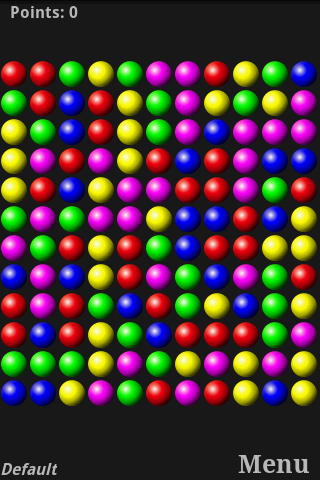
\includegraphics[scale=0.25]{bubble.png}
    \\
    \emph{figure.1}
\end{center}

A tile is said \textbf{adjacent} to another if it lies immediately (up or down or 
left or right) to another tile. Two adjacent tiles are said be \textbf{(adjacent) neighbors} if they are same in color.
Non-adjacent tiles can also be \textbf{neighbors} if starting from one we can reach another by following adjacent
neighbors only. A \textbf{cluster} is as defined as a group of same colored tiles which are neighbors to one another.
If a tile is not neighbor to any other tile then it is not a part of any cluster i.e no cluster can be of size one.
Each cluster has a score associated with it which depends on the number of tiles in this cluster. In some versions of
game, points(score) also depends upon the shape of cluster but I will only take into account the number of tiles in the cluster.
A cluster which contains n number of tiles will have n\textsuperscript{2} points(score) to award. The idea behind using 
n\textsuperscript{2} points(score) to be associated with a cluster is that score for x-sized cluster should be more than the 
sum of scores of y-sized cluster and z-sized cluster where x = y + z and 2 $\leq$ y,z $\leq$ x. It is an incentive for
player to go for larger sized clusters.Player can burst a cluster to get points(score) corresponding to it, making the tiles 
included in this cluster colorless. Game is played until board is completely empty or it reaches a state where no cluster is 
present. Aim is simple, score as high as you can.

The board has \textbf{color magnets} attached to it at its bottom and right. What these color magnets do is they attract colors 
to them if they can i.e if a colorless tile exits between a colored tile and bottom of the board then this color shift down to this 
colorless tile leaving previously colored tile colorless. Right magnet behaves in similar way but it acts on the whole column only
i.e if and only if a column of tiles is fully colorless and it has colored tiles to its left than these colored tiles will be 
shifted right by a column.

Finding an optimal solution in this game is quite a challenging problem, mainly because the search space is too large and dynamic
for traditional search methods. We can think of search space as a tree as shown in figure.2 with root node (black node) being the
starting state of the board. In this state we have a lot of clusters that we can blast providing us with number of next possible 
states as yellow state, orange state, white state and so on and same goes for these states resulting in the a tree for us to search
for best possible path to follow in order to achieve best score. We can reach same state somewhere inside the tree by following 
more than one path, for example, two paths shown in figure.2 from black state to violet state. These variety of possibilities and
their dynamic nature results in a very large search space. For a board of size 25 X 25 with 4 different possibilities for colors 
results in search space with of the order 10\textsuperscript{110} on an average. You can imagine from above example, how large 
this search space actually  is.

\begin{center}
    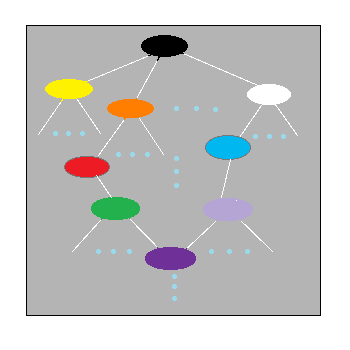
\includegraphics[scale=0.25]{tree.png}
    \\
    figure.2 
\end{center}

I will be using various strategies in which this game can be played and compare the performance of
these based on many random inputs given to them.

In Bubble Break the problem to determine whether an initially filled board can be emptied or not is NP-complete as proven in [1].

%------------------------------------------------

\section{Methods}

In this section, I describe various methods used to solve this game.
\begin{enumerate}
\item Breaking Random clusters at each step
\item Breaking largest cluster first, starting from top/bottom
\item Breaking smallest clusters first, starting from top/bottom
\item Breaking smallest clusters associated with minimum color first, starting from top/bottom
\item Breaking largest clusters associated with minimum color first, starting from top/bottom
\end{enumerate}

The first method, Breaking Random cluster at each step, is pretty simple. Select a random cluster out of all the clusters possible
in the current state of board and burst it. Keep doing this until board reaches a state with no cluster. The idea of using random 
method in one of our strategies is provide a benchmark to our comparisons of other strategies. Every other strategy's performance
will be measured with respect to this method. As it turned out from analysis, random breaking is not a very good strategy to play
this game.

The second method is a greedy-approach and it goes like this: Break the cluster which is largest in size, greedily. Because, 
largest cluster is being broken at each step of game this approach seems to be a good method
to play the game and it should result in the good score. Let's see what difference does it make if we start breaking clusters
preferably from top or bottom. Observe that there can be more than one cluster having largest size. So how to decide which one 
should you break first or it does not matter which we choose. Let A,B,C are the three largest cluster in a state S of the board.
A is located at bottom, B is above A and C lies above both A and B. If you choose to break A first then it may disturb cluster B and
cluster C by reducing or increasing their size and thus increasing the dynamic nature of the game. This disturbance can be 
considerable sometimes. If we choose to break C first then it will not have much effect on clusters A and B. But clusters A,B,C 
need not always be above or below each other, they can be left or right to each other in which case order will have least effect. 
Clusters A, B, and C can also be entwined sometimes, in these cases it can be difficult to decide which one to break first, which 
gives us yet another strategy to use, breaking clusters A, B, and C randomly.

In third approach, breaking smallest clusters first seems to be very counter-intuitive but the idea behind this is that by breaking 
smaller sized clusters first we can make the larger cluster more large i.e we are sort of trying to accumulate the larger clusters
with other clusters in order to achieve higher score as compared to when these accumulated clusters were broken individually. It is
like planning to score good in future by sacrificing some in earlier steps. We will see how this strategy works with respect to above
mentioned greedy approach. This strategy will also have variations like starting from top or bottom.

In our fourth approach idea of third approach is extended to color-distribution also. Rather than breaking smallest cluster only,
we see which color is very less in number in the board and start breaking smallest clusters corresponding to that cluster. Because by 
doing this we increase the probability of accumulation of color which is most in number and because number of tiles having this
color are more, it will result in clusters of larger sizes. This approach seems to have a little edge on third approach.

In this approach we mix the idea of fourth approach and greedy (second) approach. We start breaking clusters related to color which
is less in number but instead of small sized clusters we break larger sized clusters first. It is like being greedy but keeping it 
in check. It will also result in accumulation of color which is more in number into larger sized clusters. It is difficult to analyze
which of the fourth and fifth approach will be better on the basis of logic only. We will see how result of our simulation comes out
to be.
%------------------------------------------------

\section{Results}

The results shown in tables below are based on the simulation of bubble break game based on different strategies mentioned above. 
Size denotes the size of board on which simulations were done. Iterations is number of different simulation done on different 
boards. The starting state of board is generated randomly.
Average Score denotes the average of scores of all the hundred simulations run on 25 X 25 board with 4 colors. Number of Steps 
taken to solve the game is number of clusters broken or the number of choices made in the tree of possibilities as mentioned before
to reach the bottom (leaf node) of tree.

I have used three different cases for comparison between two methods. First case is when board size is 25 X 25 and number of colors 
are 4. This case is treated a normal case where number of clusters and their distribution across colors is almost even. In second 
case when board size is 25 X 25 and number of colors are 6 refers to the types of boards where cluster distribution may or may not 
be even and also number of clusters in starting state of board are considerably less than first case. Thus, game should be played in
order to build new clusters to score more points. In third case, board with size 35 X 35 is used with mere 4 different colors. 
In this case number of clusters is very large. Thus strategy, should not only use existing clusters carefully but also it should 
also keep on generating new clusters in order to score more points. 

These strategies provide sufficient variation to measure the difference between any two methods described above.

%--------------------------
\begin{table}[H]
\caption{}
\centering
Size = 25 X 25	\\
Iterations = 100\\
Number of colors = 4	\\

\begin{tabular}{l | c | r}
\toprule
Method & I & II \\
\hline
Average Score & 3957 & 3743 \\
\hline
Average Steps & 156 & 120 \\
\hline
\bottomrule
\end{tabular}
\end{table}

\begin{table}[H]
\caption{}
\centering
Size = 25 X 25	\\
Iterations = 100\\
Number of colors = 6	\\

\begin{tabular}{l | c | r}
\toprule
Method & I & II \\
\hline
Average Score & 1771 & 1941 \\
\hline
Average Steps & 192 & 163 \\
\hline
\bottomrule
\end{tabular}
\end{table}
\begin{table}[H]
\caption{}
\centering
Size = 35 X 35	\\
Iterations = 100\\
Number of colors = 4	\\

\begin{tabular}{l | c | r}
\toprule
Method & I & II \\
\hline
Average Score & 8570 & 8111 \\
\hline
Average Steps & 299 & 218 \\
\hline
\bottomrule
\end{tabular}
\end{table}

As from the Tables above it is clear our greedy approach works just as good as random method which implies it is not a good way to
play the game. It uses much less steps to complete the game which is clear from the fact that at every step this method eliminates
more number of colored tiles than random strategy. Hence it will reach the end earlier than random method.

%--------------------------

\begin{table}[H]
\caption{}
Size = 25 X 25	\\
Iterations = 100\\
Number of colors = 4	\\
\centering
\begin{tabular}{l | c | r}
\toprule
Method & I & III \\
\hline
Average Score & 3920 & 7181 \\
\hline
Average Steps & 156 & 189 \\
\hline
\bottomrule
\end{tabular}
\end{table}

\begin{table}[H]
\caption{}
Size = 25 X 25	\\
Iterations = 100\\
Number of colors = 6	\\
\centering
\begin{tabular}{l | c | r}
\toprule
Method & I & III \\
\hline
Average Score & 1749 & 2086 \\
\hline
Average Steps & 191 & 219 \\
\hline
\bottomrule
\end{tabular}

\end{table}
\begin{table}[H]
\caption{}
Size = 35 X 35	\\
Iterations = 100\\
Number of colors = 4	\\
\centering
\begin{tabular}{l | c | r}
\toprule
Method & I & III \\
\hline
Average Score & 8726 & 20038 \\
\hline
Average Steps & 299 & 378 \\
\hline
\bottomrule
\end{tabular}
\end{table}

From Table 4, 5, 6 we can see that third method is much better than random one and consequently better than the second method (greedy)
method. Hence, our assumption that breaking smaller clusters first will result in larger cluster later in the game turned out to be
right. Score obtained by method III is almost twice than the random method. The approach which was very counter-intuitive turned out 
to be much better than a simple approach (greedy) based on intuition. As we can see from Table 6 this strategy is pretty good at 
using existing larger clusters to score but if we consider Table 5, this strategy is not very good at generating large clusters when 
there are not any. It ends up using many smaller clusters rather than forming a bigger cluster using them. This method also takes 
much more steps to completely solve the game as at every step it eliminates less number of tiles than random method.

%----------------------------

\begin{table}[H]
\caption{}
Size = 25 X 25	\\
Iterations = 100\\
Number of colors = 4	\\
\centering
\begin{tabular}{l | c| r}
\toprule
Method & I & IV \\
\hline
Average Score & 4061 & 20360 \\
\hline
Average Steps & 156 & 149 \\
\hline
\bottomrule
\end{tabular}
\end{table}

\begin{table}[H]
\caption{}
Size = 25 X 25	\\
Iterations = 100\\
Number of colors = 6	\\
\centering
\begin{tabular}{l | c| r}
\toprule
Method & I & IV \\
\hline
Average Score & 1736 & 3117 \\
\hline
Average Steps & 192 & 188 \\
\hline
\bottomrule
\end{tabular}

\end{table}
\begin{table}[H]
\caption{}
Size = 35 X 35	\\
Iterations = 100\\
Number of colors = 4	\\
\centering
\begin{tabular}{l | c| r}
\toprule
Method & I & IV \\
\hline
Average Score & 8655 & 86881 \\
\hline
Average Steps & 299 & 291 \\
\hline
\bottomrule
\end{tabular}
\end{table}

Fourth Strategy seems to be beating every other method so far as we can confirm from the data provided in the tables. This strategy 
is far far better than the random one. Not only it used existing blocks very well (refer to Table 9) but it also did much better 
than the third strategy when there was scarcity of clusters (refer to Table 8). This strategy did exactly what we expected. As it was extension of 
third strategy where only smallest cluster was eliminated but here we eliminated smallest clusters corresponding to minimum color
which helped color ,which was larger in number, to form larger clusters in the mean time.

%-----------------------------
\begin{table}[H]
\caption{}
Size = 25 X 25	\\
Iterations = 100\\
Number of colors = 4	\\
\centering
\begin{tabular}{l | c| r}
\toprule
Method & I & V \\
\hline
Average Score & 4045 & 3122 \\
\hline
Average Steps & 155 & 177 \\
\hline
\bottomrule
\end{tabular}
\end{table}

\begin{table}[H]
\caption{}
Size = 25 X 25	\\
Iterations = 100\\
Number of colors = 6	\\
\centering
\begin{tabular}{l | c| r}
\toprule
Method & I & V \\
\hline
Average Score & 1762 & 1415 \\
\hline
Average Steps & 190 & 200 \\
\hline
\bottomrule
\end{tabular}
\end{table}

\begin{table}[H]
\caption{}
Size = 35 X 35	\\
Iterations = 100\\
Number of colors = 4	\\
\centering
\begin{tabular}{l | c| r}
\toprule
Method & I & V \\
\hline
Average Score & 8795 & 7290 \\
\hline
Average Steps & 299 & 351 \\
\hline
\bottomrule
\end{tabular}
\end{table}

In this strategy, we were eliminating largest clusters corresponding to the color which was minimum in number. It turns out that 
keeping the greed in check also do not help. As clear from the data this method is performing poorer than the random strategy. The
reason can be the even distribution of clusters among colors in the examples we took. Because if distribution of clusters is even 
than this method should work more or less same as second method, which it did.

So, let us compare strategy IV and V on a board with uneven distribution of colors.

\begin{table}[H]
\caption{}
Color Distribution: Uneven\\
Size = 25 X 25	\\
Iterations = 100\\
Number of colors = 4	\\
\centering
\begin{tabular}{l | c| r}
\toprule
Method & I & IV \\
\hline
Average Score & 36077 & 65471 \\
\hline
Average Steps & 51 & 62 \\
\hline
\bottomrule
\end{tabular}
\end{table}

\begin{table}[H]
\caption{}
Color Distribution: Uneven\\
Size = 25 X 25	\\
Iterations = 100\\
Number of colors = 4	\\
\centering
\begin{tabular}{l | c| r}
\toprule
Method & I & V \\
\hline
Average Score & 39660 & 1157 \\
\hline
Average Steps & 50 & 46 \\
\hline
\bottomrule
\end{tabular}
\end{table}

Even when color distribution is uneven method V worked pretty badly as compared to random strategy (refer to table 14). But Strategy
IV worked still better than the random strategy. Thus method V is not a very good method to play the game of Bubble Break. The reason 
for method V to perform poorly is mainly because it lacks planning accumulation of clusters in the future steps, which is exactly the
reason why method IV is perform better than other algorithms.

%------------------------------------------------

\section{Discussion}

Developing an algorithm for to find an optimal solution in Bubble Break game is not easy. The search space for solving this game 
is very large and dynamic for traditional search methods to exhaust all the possibilities in practical time. Thus, we need to come 
up with some different strategy in order to find solution to this game. Some simple strategies to solve this game are discussed and 
compared above. These strategies do not find an optimal solution to this game still some of these strategies work much better than 
random finding a solution to the game. There can be lots of other strategies possible similar to those mentioned above like 
eliminating smaller clusters corresponding to maximum color first or keeping the maximum color and using method III on rest of the 
colors. But method IV works much better than all these strategies mentioned on an average. This strategy works on the principle of
bringing together smaller clusters to form larger clusters at as little expense as possible in order to use these larger clusters
later in the game. Memory (remembering the previous configurations of board while playing game) can play an important role in 
developing a still better algorithm using strategy IV. In that case we can revert back some steps in order to select that state of
board which will result in better score later in the game.

%----------------------------------------------------------------------------------------
%	REFERENCE LIST
%----------------------------------------------------------------------------------------

\begin{thebibliography}{99} % Bibliography - this is intentionally simple in this template

[1] T. Biedl, E. Demaine, M. Demaine, R. Fleischer, L. Jacobsen and J. Ian Munro. The complexity of

Clickomania. In More Games of No Chance, pages 389 to 404, Cambridge University Press, 2002.\\

[2] Frank W. Takes, Walter A. Kosters. Solving SameGame and its Chessboard Variant. 

Leiden Institute of Advanced Computer Science, Leiden University, The Netherlands\\

http://www.liacs.nl/~kosters/samegame.pdf

\end{thebibliography}

%----------------------------------------------------------------------------------------

\end{multicols}

\end{document}
